
\subsection{NUCache}
\label{sec:algorithms:nucache}

\begin{figure}[ht]
    \centering
    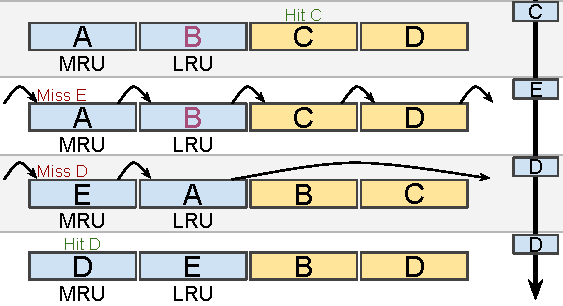
\includegraphics[width=.65\textwidth]{figures/algorithms/NUCache}
    \caption[NUCache managed 4-way cache set.]{NUCache managed 4-way cache set. (M=2)}
    \label{fig:algorithms:nucache_example}
\end{figure}

Next Use Cache (NUCache)~\cite{Manikantan2011} was first proposed in 2011.
NUCache does not partition the cache by examining each core's access pattern separately like many of the other algorithms. 
Instead, NUCache uses the concept of delinquent PCs.
A delinquent PC is the PC value of a memory instruction that often causes cache misses.
By evaluating the properties of the delinquent PCs, NUCache selects a set of PCs and allocates more cache space to blocks loaded by these instructions.
Because all applications running may contain one or more delinquent PCs, NUCache will implicitly share the cache between the applications.

To detect delinquent PCs, NUCache uses a novel DeliTrack structure.
The DeliTrack is a storage structure, indexed by PC that stores a miss count, insertion time and a next use histogram. 
LRU is used to manage the DeliTrack, which naturally ensures that PCs causing many misses are kept while others are replaced.
The next use histogram counts the next use value of blocks loaded into the cache by the given PC in buckets of 8 from 0 to 64.
This histogram is later used when a set of prioritized delinquent PCs are selected.

The next use distance of a block is defined as the number of misses observed by the cache between the time the block was evicted and the next time it is loaded due to a cache miss.
This number is then scaled by the number of sets in the cache to get the set relative next use distance.
An additional storage structure, NUTrack, is used to generate the next use histogram in the DeliTrack.
NUTrack is a set-associative structure indexed by block address.
Each row in the NUTrack stores a evicted bit, eviction time, and PC.
When a new block belonging to a PC in the DeliTrack is inserted into the cache, an attempt is made to insert a new row in the NUTrack. 
A row is inserted iff there is a valid replacement target in the NUTrack.
Two valid replacements exists; an unused row, or a row with the eviction bit set to true and an eviction time older than the maximum tracked next use value (64).
When a block is evicted from the main cache, the eviction bit and eviction time is set in the corresponding NUTrack row, if it exists.
On insertion in the main cache, the NUTrack searches for a matching row. 
If a matching row exists the next use distance is calculated and if the value is lower than the max value (64) the corresponding row in the DeliTrack histogram is incremented.

NUCache divides the ways in each cache set into two groups, MainWays, and DeliWays.
The MainWays are managed by LRU while the DeliWays are simply first in first out.
The value $M$ defines the number of DeliWays.
NUCache attempts to reduce misses by not evicting blocks from selected delinquent PCs when they are evicted from the MainWays, but rather let them enter the DeliWays.
By using the size of the DeliWays and the next use information in the DeliTrack structure, the algorithm periodically selects a set of PCs that are allowed to use the DeliWays.
The selection is done using a greedy algorithm that attempts to ensure that each block entering the DeliWays will receive a hit at least once before they are pushed out by other blocks.
DeliWays and MainWays are implemented by having two extra bits per cache block, one indicating if the block can enter the DeliWays, another indicating if the block is the DeliWays.
On insertion, all blocks inserted into to the MainWays.
When the LRU block in the MainWays is about to be replaced, the algorithm checks if it is marked to enter the DeliWays.
If the block is allowed to enter the DeliWays, it will not be evicted but rather moved from the MainWays.
If, after moving the new block into the DeliWays, the number of DeliWays blocks has exceeded $M$ the oldest block is removed.
Otherwise, the new LRU block in the MainWays is evaluated.
Because of this implementation the MainWays may use the entire cache if no DeliWays are in use, at the same time the DeliWays cannot exceed $M$.
This allows for an efficient use of every cache set.

Figure~\ref{fig:algorithms:nucache_example} shows an example cache set managed by NUCache with M set to 2.
Initially, there are four blocks, A, B, C, and D.
A and B are in the MainWays, indicated by the blue background.
While, C and D are in the DeliWays, as indicated by the yellow background.
Block B is eligible for insertion into the DeliWays, no other blocks in the example are eligible for the DeliWays.
The first request is for block C, this is a hit.
C is not promoted as it is a part of the FIFO managed DeliWays.
Next is a request for E, and this is a miss.
The cache first attempts to evict B, but B is eligible for DeliWays and is not evicted.
After B enters the DeliWays, it contains a total of 3 blocks, this is one more than the upper limit of 2, and hence the first in, D, is evicted.
E is then inserted at the MRU position.
Next is a request for D; this is also a miss, and A at the LRU position is evicted.
The final request is also for D, causing no change as D is already at the MRU position.

